\chapter{Problematyka zagadnienia}
\label{ch:problematyka}

%---------------------------------------------------------------------------
\section{Charakterystyka choroby Parkinsona}
\label{sec:charakterystykaPD}

Choroba Parkinsona (ang. \emph {Parkinson Disease,  PD}) to zwyrodnieniowe schorzenie mózgu, które wiąże się z objawami ruchowymi, takimi jak spowolnienie ruchowe,
drżenie, sztywność oraz zaburzenia chodu i równowagi.
Ponadto może prowadzić do różnorodnych powikłań niemotorycznych, obejmujących zaburzenia poznawcze, stany psychiczne,
trudności ze snem oraz dolegliwości sensoryczne, w tym ból.
Początkowe objawy często rozwijają się stopniowo, nasilając się w miarę upływu czasu.
Postęp choroby prowadzi do znacznego stopnia niepełnosprawności, co może wymagać wsparcia i opieki.
U wielu osób zdiagnozowanych z chorobą Parkinsona występują także zmiany w sferze psychicznej i behawioralnej, takie jak
trudności ze snem, depresja, problemy z pamięcią oraz uczucie przewlekłego zmęczenia.

\begin{figure}[htbp]
	\centering
	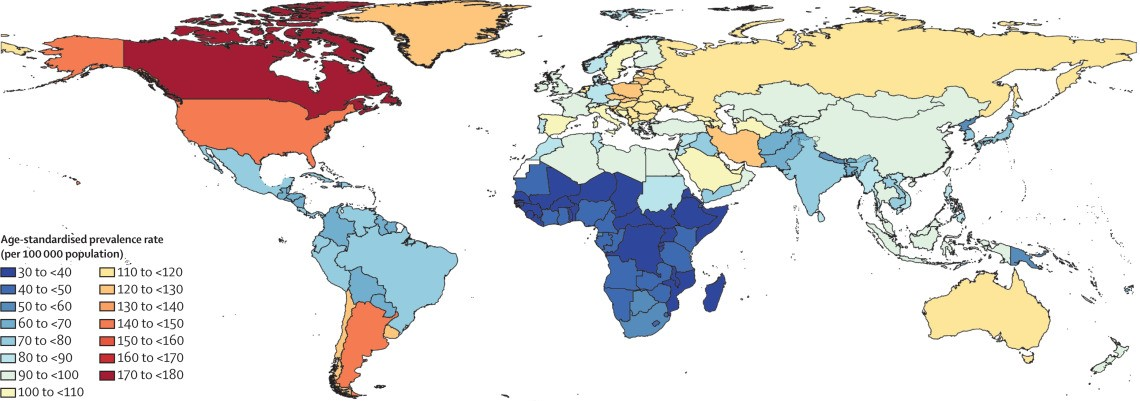
\includegraphics[width=0.9\textwidth]{./img/map}
	\caption{Choroba Parkinsona na świecie \cite{global_PD}}
    \label{fig:PD_map}
\end{figure}

Zgodnie z danymi przedstawionymi w raporcie Światowej Organizacji Zdrowia \cite{WHO}, choroba Parkinsona (PD) stanowi obecnie narastający problem na skalę światową. Zarówno wskaźniki niepełnosprawności, jak i zgony związane z tą chorobą rosną szybciej niż w przypadku innych zaburzeń neurologicznych.

W ciągu ostatnich 25 lat zaobserwowano podwojenie częstości występowania PD na całym świecie.
Globalne szacunki na rok 2019 wskazują, że liczba osób cierpiących na PD przekroczyła 8,5 miliona.
Co więcej, analizy obrazują, że w 2019 roku choroba spowodowała aż 5,8 miliona lat życia z niepełnosprawnością, co oznacza wzrost o 81\% w porównaniu z danymi z roku 2000.
Jednocześnie liczba zgonów związanych z PD wyniosła 329 000, co stanowi wzrost o ponad 100\% w porównaniu z rokiem 2000 \cite{global_PD}.
W Polsce z chorobą Parkinsona zmaga się około 100 tys. pacjentów, z czego około 20\% jest już w stadium zaawansowanym
według informacji przekazywanych przez Fundację Chorób Mózgu.
Ponadto co roku w naszym kraju wykrywanych jest ok. 8 tys. nowych zachorowań.

PD jest istotną sprawą dotyczącą zdrowia publicznego, ponieważ jej częstotliwość występowania związana jest ze zjawiskiem starzejącego się społeczeństwa.
Razem z innymi chorobami neurodegeneracyjnymi, takimi jak choroba Alzheimera, ma szanse stać się drugą zaraz za nowotworami przyczyną zgonów do 2040 roku (WHO).

Przyczyna PD nie jest znana, ale uważa się, że powstaje w wyniku złożonej interakcji pomiędzy czynnikami genetycznymi i
narażeniem na czynniki środowiskowe, takie jak pestycydy, rozpuszczalniki i zanieczyszczenia powietrza.
Niektóre przypadki wydają się dziedziczne, a kilka można przypisać określonym wariantom genetycznym.
Chociaż uważa się, że genetyka odgrywa rolę w chorobie Parkinsona, w większości przypadków choroba nie występuje rodzinnie \cite{National_Institute_on_Aging_2022}.

\begin{figure}[htbp]
	\centering
	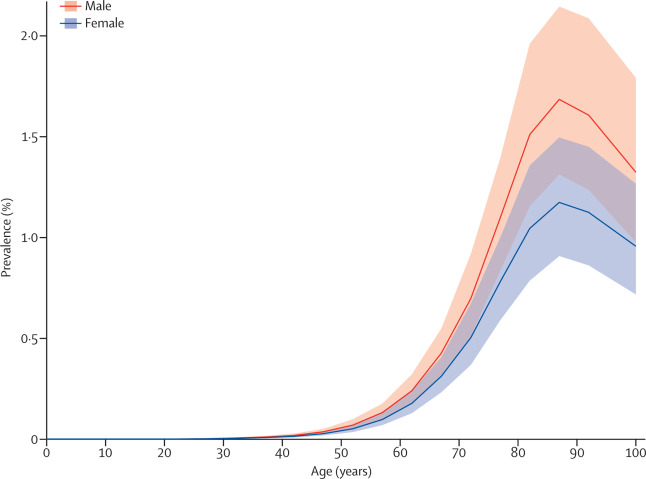
\includegraphics[width=0.6\textwidth]{./img/PD_prevalence}
	\caption{Rozpowszechnienie choroby Parkinsona w zależności od wieku \cite{global_PD}}
    \label{fig:PD_prevalance}
\end{figure}

Mimo że każdy może być narażony na ryzyko rozwoju choroby Parkinsona, to częściej występuje ona u mężczyzn niż u kobiet,
a wiek stanowi kluczowy element wpływający na ryzyko zachorowania, co można zobaczyć na Rys.\ref{fig:PD_prevalance}.
Statystyki pokazują, że ryzyko zachorowania rośnie wraz z wiekiem, chociaż choroba może dotyczyć także młodszych osób (nawet w wieku 20 lat).
U większości pacjentów po raz pierwszy choroba rozwija się po 60 roku życia, około 5\% do 10\% doświadcza jej początku przed 50 rokiem życia.
Postacie choroby Parkinsona o wczesnym początku są często, choć nie zawsze, dziedziczne i niektóre formy zostały powiązane z
określonymi zmianami w genach \cite{National_Institute_on_Aging_2022}.

%---------------------------------------------------------------------------

\subsection{Objawy choroby}
\label{subsec:objawy}

Najbardziej widoczne oznaki i objawy choroby Parkinsona pojawiają się, gdy komórki nerwowe w zwojach podstawy mózgu,
obszarze mózgu kontrolującym ruch, ulegają uszkodzeniu i/lub obumierają.
Zwykle te komórki nerwowe lub neurony wytwarzają dopaminę.
Kiedy neurony obumierają lub ulegają uszkodzeniu, wytwarzają mniej dopaminy, co powoduje problemy z poruszaniem się
związane z chorobą.
Na ten moment nie wiadomo co powoduje śmierć neuronów.
Zanikają również zakończenia nerwowe, które wytwarzają norepinefrynę, główny przekaźnik chemiczny
współczulnego układu nerwowego, który kontroluje wiele funkcji organizmu, takich jak tętno i ciśnienie krwi.
Utrata norepinefryny może pomóc wyjaśnić niektóre cechy choroby Parkinsona związane z brakiem ruchu, takie jak zmęczenie,
nieregularne ciśnienie krwi, zmniejszony ruch pokarmu w przewodzie pokarmowym i nagły spadek ciśnienia krwi, gdy osoba wstaje z pozycji siedzącej lub leżącej.

\vspace{0.5cm}
Do czterech głównych objawów choroby Parkinsona zalicza się:
\begin{itemize}[itemsep=0.05pt]
	\item drżenie rąk, ramion, nóg, szczęki lub głowy,
	\item sztywność mięśni, gdy mięśnie pozostają skurczone przez długi czas,
	\item powolność ruchu,
	\item zaburzenia równowagi i koordynacji, czasami prowadzące do upadków.
\end{itemize}

\vspace{0.15cm}
Pozostałe objawy mogą obejmować:
\begin{itemize}[itemsep=0.05pt]
	\item depresja i inne zmiany emocjonalne,
	\item trudności w połykaniu, żuciu i mówieniu,
	\item problemy z układem moczowym lub zaparcia,
	\item problemy skórne.
\end{itemize}


Objawy choroby Parkinsona oraz tempo jej postępu mogą znacząco różnić się wśród poszczególnych osób.
Na wczesnym etapie choroby objawy są subtelne i kształtują się stopniowo.
Często zaczynają się od jednej strony ciała lub nawet jednej kończyny.
W miarę jak choroba rozwija się, dotyka ona ostatecznie obu stron, jednak niekiedy objawy mogą być bardziej intensywne po jednej stronie niż po drugiej.
Niektórzy pacjenci z chorobą Parkinsona doświadczają pewnych zwiastunów przed wystąpieniem charakterystycznych cech, takich jak sztywność czy drżenie.
Mogą to być trudności ze snem, problemy z wypróżnianiem, utrata węchu czy także zespół niespokojnych nóg.
Warto jednak zaznaczyć, że niektóre z wymienionych objawów mogą również występować w procesie naturalnego starzenia się \cite{National_Institute_on_Aging_2022}.


Chociaż tempo postępu choroby Parkinsona zazwyczaj jest powolne, w końcu ma to wpływ na codzienne funkcjonowanie osoby dotkniętej tą dolegliwością.
Wykonywanie zwykłych czynności, takich jak praca, prowadzenie domu czy uczestnictwo w spotkaniach towarzyskich z przyjaciółmi, może stawać się wyzwaniem.

%---------------------------------------------------------------------------

\section{Znaczenie głosu}
\label{sec:znaczenie_glosu}
Choroba Parkinsona, będąca rezultatem zaburzonej funkcji układu nerwowego, wywołuje objawy w różnych obszarach ciała.
W przypadku choroby Parkinsona objawy zaburzeń mowy powodowane są przede wszystkim przez deficyt czynnościowy krtani, zmniejszoną pojemność życiową płuc,
osłabioną pracę mięśni mimicznych oraz zmiejszony napęd mówienia \cite{lewicka}.
Zwykle stają się widoczne w średniozaawansowanym stadium schorzenia, co oznacza, że przez długi okres mowa pozostaje relatywnie nienaruszona.
Rozpoznanie tych zaburzeń może być niekiedy trudne, gdyż wymaga odróżnienia, czy powstały one na skutek samej choroby, czy też są rezultatem naturalnego
procesu starzenia się organizmu.
Proces starzenia wpływa na fizjologiczne osłabienie słuchu, co z kolei może prowadzić do zmian w brzmieniu głosu.
Głos staje się osłabiony, wykazujący tendencję do drżenia, a także jego zakres tonacji może ulec zawężeniu.

Objawy zaburzeń mowy i głosu związane z chorobą Parkinsona nie są łatwo dostrzegalne dla osób bez specjalistycznej wiedzy w tej dziedzinie.
Przeważnie zdolność rozumienia mowy pozostaje niezmieniona.
Niemniej jednak, w trakcie spontanicznych wypowiedzi pacjenci zaczynają ograniczać ilość przekazywanych informacji i mogą napotykać trudności w składaniu
pełnych zdań.
Te trudności nie wynikają koniecznie z ubytku słownictwa, ale raczej z nieprawidłowego doboru słów.
Wskazujące na podłoże chorobowe objawy obejmują między innymi \cite{Szurek_2018, Kuryłowicz_2019}:
\begin{itemize}[itemsep=0.1pt]
	\item mowę powolną, monotonną i przerywaną,
	\item nadmierne ślinienie się,
	\item niewyraźną i zamazaną artykulację,
	\item skrócony czas fonacji
	\item chuchający i tremolujący głos
	\item spłaszczoną barwę i obniżone natężenie
	\item niewłaściwą koordynację mięśni nasady, które mogą być zwiotczałe lub zbyt napięte,
	\item czasami przyspieszenie tempa wypowiedzi w jej końcowej fazie, co może utrudnić zrozumienie pacjenta.
\end{itemize}

Te objawy pojawiają się w średniozaawansowanym stadium choroby, są wystarczająco wyraźne, aby mogły zostać zauważone słuchowo przez specjalistów.
Niemniej jednak badania wskazują, że istnieją subtelne zmiany w głosie, które pojawiają się jeszcze wcześniej, nawet w fazie przedobjawowej \cite{2023_PD_voice}.

W roku 2000 przeprowadzono badanie akustyczne i percepcyjne cech głosu pacjentów z chorobą Parkinsona, zależnie od stopnia nasilenia choroby \cite{https://doi.org/10.1080/136828200410654}.
W nagraniach głosowych, składających się z przedłużonej samogłoski /a/, śpiewu gamy oraz 1-minutowego monologu, stwierdzono, że głosy pacjentów z PD,
zarówno we wczesnych, jak i późniejszych stadiach choroby, charakteryzowały się ograniczoną percepcyjnie zmiennością tonu i głośności, chropowatością
oraz zmniejszoną głośnością.

Wspomniane badanie sugerowało również, że głosy pacjentów z PD wykazywały nadmierne drganie, wysoką częstotliwość podstawową (szczególnie u mężczyzn) oraz zmniejszoną zmienność częstotliwości podstawowej (szczególnie u kobiet).
Część z tych cech głosu nie wydawała się pogarszać w miarę postępu choroby, jednak cechy takie jak oddech, monotonność i jednolitość mowy, niska głośność oraz ograniczony maksymalny zakres częstotliwości fonacyjnej były bardziej zauważalne w późniejszych stadiach choroby Parkinsona.

Podobne badanie przeprowadzone przez Gamboę i innych (1997) wykazało, że w porównaniu z grupą kontrolną, pacjenci z PD wykazywali wyższy jitter, niższy stosunek harmonicznych do szumów (H/N), mniejszą zmienność częstotliwości i intensywności mowy, niższy zakres fonacyjny oraz wyższą częstotliwość obecności głosu o niskim natężeniu, jednotonowość i zatrzymanie głosu.
Wskazano również, że te cechy nie wykazywały znaczącego związku z czasem trwania choroby \cite{GAMBOA1997314}.

Mnogość objawów, które są zauważalne w głosie, motywuje do uzwględnienia ich w diagnostyce.
Prowadzone są badania, które wykorzystują analizę mowy do wykrywania patologii i schorzeń związanych z narządem głosu, takich jak ostre zapalenie krtani czy porażenie nerwu krtaniowego wstecznego.
Może to w przyszłości pozwolić na identyfikację problemów zdrowotnych, na przykład wśród osób pracujących głosem, jak nauczyciele, bez konieczności inwazyjnych badań gardła.
Podobne podejście można zastosować do diagnozowania i monitorowania chorób neurodegeneracyjnych.
Badania naukowe wskazują, że analiza głosu może stanowić podstawę dla automatycznej diagnostyki oraz monitorowania choroby Parkinsona.

Takie podejście niesie za sobą wiele korzyści, które mogą rewolucjonizować sposób diagnozowania oraz monitorowania tej neurodegeneracyjnej choroby.
W kontekście diagnostyki choroby Parkinsona, analiza głosu stanowi innowacyjne podejście, skupiające się na mowie i jakości głosu pacjenta.
Głos, będący wskaźnikiem stanu układu nerwowego i zdolności komunikacyjnych, dostarcza szeroką gamę informacji kluczowych dla procesu diagnozowania.
Różnorodność parametrów akustycznych i fonacyjnych, które można zbadać, otwiera drzwi do kompleksowej oceny zmian zachodzących w organizmie pacjenta.

Wczesne objawy choroby Parkinsona często bywają trudne do wykrycia, szczególnie w standardowych badaniach klinicznych.
Analiza głosu pozwala na szybką identyfikację subtelnych zmian, które pojawiają się we wczesnych fazach choroby.
Ta wczesna detekcja umożliwia natychmiastową interwencję terapeutyczną, co może wpłynąć na spowolnienie progresji choroby i poprawę jakości życia pacjenta.

Analiza głosu jako narzędzie diagnostyczne wprowadza nowe perspektywy dla specjalistów zajmujących się chorobą Parkinsona.
Logopedzi, foniatrzy i lekarze mogą wykorzystać obiektywne dane akustyczne do dokładnej oceny zmian w mowie i jakości głosu pacjenta.
To również umożliwia ocenę stanu pacjenta oraz sugerowanie odpowiednich interwencji, włącznie z dostosowaniem leczenia farmakologicznego.

Dla pacjentów analiza głosu oznacza bardziej konkretne oceny ich stanu i dostosowane terapie, przyczyniające się do zwiększenia efektywności procesu leczenia.
Analiza głosu, jako nieinwazyjne badanie, skraca czas oceny pacjenta.
Badanie to jest szybkie, wygodne i bezpieczne, co może zachęcać pacjentów do systematycznego uczestnictwa w procesie diagnostycznym.
Wprowadza to szczególną wartość dla pacjentów, którym trudno się przemieszczać.

Analiza głosu jako narzędzie diagnostyczne przy chorobie Parkinsona otwiera drzwi ku nowym, zaawansowanym metodologiom diagnozowania i leczenia,
które mogą mieć znaczący wpływ na poprawę jakości życia pacjentów.
Dodatkowo może być wykorzystana do oceny stanu pacjenta oraz sugerowania odpowiednich interwencji, włączając zmiany w leczeniu farmakologicznym.
W konsekwencji ma potencjał stania się szybkim, nieinwazyjnym wsparciem diagnostycznym i terapeutycznym, przyczyniając się do polepszenia
opieki nad pacjentami dotkniętymi chorobą Parkinsona.

%---------------------------------------------------------------------------
\section{Metody diagnozowania i monitorowania}
\label{subsec:diagnostyka}

Diagnostyką choroby Parkinsona zajmują się neurolodzy i geriatrzy.
Jej rozwój jest długotrwały, a w początkowych latach klinicznie niemal niewidoczny, co utrudnia wczesne rozpoznanie.
Subtelne objawy często są uważane za skutek starzenia się lub błędnie diagnozowane jako inne zaburzenia neurologiczne.
Kluczowym elementem w tym stadium jest dokładny wywiad, badanie fizykalne oraz identyfikacja objawów przez lekarza.
Następnie diagnoza jest rozwijana poprzez badania laboratoryjne  oraz obrazowe.
Niestety, wyniki tych badań rzadko potwierdzają diagnozę od razu.

Początkowo pacjent zwykle konsultuje się z lekarzem pierwszego kontaktu, który powinien dokonać wstępnej diagnozy i skierować do neurologa.
W tej fazie diagnozy przeprowadza się szczegółowy wywiad, uwzględniający rodzaj, nasilenie oraz okres występowania objawów, a także
obecność chorób neurozwyrodnieniowych w rodzinie.
Neurolog przeprowadza kompleksowe badanie neurologiczne, identyfikując symptomy takie jak sztywność mięśni, ograniczenia w
ruchu (spowolnienie, trudności w poruszaniu się), drżenia spoczynkowe (np. w głowie, palcach rąk) oraz zaburzenia postawy i równowagi
(zgarbienie, niestabilność, upadki). Kolejne badania są wykonywane w celu potwierdzenia lub wykluczenia diagnozy \cite{diagnostyka_Sitek, Loscalzo_2022}.

\renewcommand{\labelenumi}{\alph{enumi})}
\begin{enumerate}
	\item Badania laboratoryjne
	\item[] Obecnie brak specyficznych badań laboratoryjnych krwi, które potwierdzałyby diagnozę choroby Parkinsona.
Niemniej jednak, takie badania są użyteczne w wykluczaniu innych chorób o podobnym przebiegu.
Wykonuje się podstawowe badania, takie jak morfologia krwi, elektrolity, poziom glukozy, TSH, próby wątrobowe, mocznik, kreatynina oraz poziom witaminy B12.

	\item Badania obrazowe
	\item[] Badania obrazowe głowy są przeprowadzane w celu wykluczenia innych chorób o podobnych objawach.
Zalicza się do nich tomografię komputerową, ultrasonografię mózgu (USG) oraz rezonans magnetyczny głowy (MRI).
Międzynarodowe kryteria rozpoznania choroby Parkinsona nie nakładają obowiązku wykonywania badań obrazowych w celu potwierdzenia diagnozy.
Dostępne są również zaawansowane techniki obrazowania, takie jak PET (pozytonowa emisyjna tomografia) oraz SPECT (tomografia emisyjna pojedynczego fotonu), które pozwalają na obserwację metabolizmu w układzie pozapiramidowym. Skan DAT (skan transportera dopaminy) jest przykładem SPECT i może być sugerowany przez specjalistę.
Mimo to, ostateczna diagnoza opiera się na objawach oraz wynikach badania neurologicznego. Większość pacjentów nie wymaga skanowania DAT.

	\item Test z lewodopą
	\item[]Test polega na podaniu pacjentowi  preparatu z lewodopą.
Jeśli następuje poprawa po zażyciu, istnieje wysokie prawdopodobieństwo, że pacjent rzeczywiście cierpi na chorobę Parkinsona.
W przypadku braku poprawy, konieczne może być dalsze rozszerzenie diagnostyki.

	\item Badania genetyczne
	\item[] Choroba Parkinsona może występować rodzinnie, co skłania do rozważenia diagnostyki genetycznej u pacjenta i jego krewnych.
Obecnie zidentyfikowano 12 mutacji genów, które mogą wpływać na ryzyko zachorowania na PD, należy jednak pamiętać, że badania genetyczne są kosztowne.

	\item Badania węchu
	\item[] Większość osób z chorobą Parkinsona (90\%) doświadcza zaburzeń węchu, manifestujących się hiposomią (osłabienie węchu), także we wczesnym stadium choroby.
Jednak nie obserwuje się tych zaburzeń w przypadku zaniku wieloukładowego i postępującego porażenia nadjądrowego.

	\item Badania neuropsychologiczne i neuropsychiatryczne
	\item[] Badania te służą identyfikacji zaburzeń poznawczych i emocjonalnych.
Celem jest diagnoza łagodnych zaburzeń poznawczych, otępienia, a także zaburzeń psychotycznych, lękowych, kontroli impulsów i depresji.
\end{enumerate}

Objawy przypominające chorobę Parkinsona są diagnozowane jako parkinsonizm i mogą być spowodowane różnymi zaburzeniami, takimi jak postępujące porażenie nadjądrowe, zanik wieloukładowy,
drżenie samoistne, demencja z ciałami Lewy'ego, choroby naczyniowe mózgu, otępienie, reumatyzm oraz inne \cite{diagnostyka_Sitek}.
Różnicowanie tych schorzeń jest kluczowe, ponieważ leczenie i podejście terapeutyczne są różne.
Chociaż ostateczną diagnozę można ustalić tylko na podstawie badania mózgu po zgonie, wcześniej zdefiniowane kryteria diagnostyczne pozwalają na dokonanie diagnozy klinicznej.
Według badania z 2021 roku \cite{ROSSI202153} diagnoza klinicznie potwierdzonej choroby Parkinsona może zabierać od kilku miesięcy do kilku lat, zależnie od indywidualnych czynników oraz reakcji na terapię lewodopą.

Pomocnym narzędziem w diagnostyce są szeroko stosowane skale oceny choroby Parkinsona.
Stanowią istotne narzędzie w monitorowaniu stanu pacjentów oraz ocenie postępów choroby.
Te strukturalne i skwantyfikowane metody pomagają lekarzom i opiekunom ocenić stopień nasilenia objawów ruchowych,
jak również wpływ choroby na codzienne funkcjonowanie pacjenta.
Popularne skale, takie jak Skala Hoehn-Yahra, Skala UPDRS (Unified Parkinson's Disease Rating Scale) oraz Skala Schwab-England,
umożliwiają stosunkowo obiektywną analizę symptomów i wsparcie w podejmowaniu decyzji terapeutycznych.
Dzięki tym narzędziom możliwe jest dostosowanie leczenia do indywidualnych potrzeb pacjenta oraz śledzenie skuteczności terapii na przestrzeni czasu.

Obecnie proces diagnozy jest wyjątkowo złożony i wieloetapowy.
W celu skutecznej identyfikacji i monitorowania pacjentów z chorobą Parkinsona, zaleca się regularne wizyty kontrolne u neurologów specjalizujących
się w zaburzeniach ruchowych.
W odpowiedzi na te wyzwania, naukowcy koncentrują się na opracowaniu bardziej efektywnych narzędzi diagnostycznych.
Poszukiwane są innowacyjne metody, które przyspieszą i usprawnią ten proces.
Rozwinięcie skuteczniejszych narzędzi diagnostycznych przyniesie korzyści nie tylko finansowe, ale także pozwoli na szybsze i trafniejsze udzielanie pomocy pacjentom cierpiącym na chorobę Parkinsona.
Poprawa diagnozy pomoże podnieść standard życia osób dotkniętych tym schorzeniem, co jest priorytetem dla społeczności medycznej i pacjentów.
W nadchodzących latach, dążenie do wypracowania bardziej efektywnych metod diagnozowania choroby Parkinsona będzie kluczowym krokiem w zapewnieniu lepszej opieki zdrowotnej i poprawie jakości życia pacjentów.

%---------------------------------------------------------------------------

\section{Terapia osób chorych}
\label{sec:terapia}
Obecnie brak jest kuracji na chorobę Parkinsona, dlatego terapia skupia się na przywracaniu pacjentom zdolności funkcjonowania
lub, w przypadkach zaawansowanych, na poprawie jakości życia.
Zgodnie z aktualnym standardem medycznym, w terapii wykorzystuje się różnorodne metody, w tym leczenie farmakologiczne, głęboką stymulację mózgu oraz rehabilitację \cite{National_Institute_on_Aging_2022}.

Leczenie farmakologiczne choroby Parkinsona opiera się na zwiększeniu poziomu dopaminy w mózgu, co wpływa na kontrolę objawów
ruchowych i niezwiązanych z ruchem. Główną terapią jest lewodopa, która jest przetwarzana przez komórki nerwowe w dopaminę.
Leczenie lewodopą często łączy się z karbidopą, która zmniejsza skutki uboczne i ilość potrzebnej lewodopy.
Stosuje się też inne terapie farmakologiczne o różnych zasadach działania m.in. pobudzające produkcję dopaminy,
zwiększające ilość dopaminy poprzez spowolnienie jej rozkładu, redukujące ruchy mimowolne czy zmniejszające drżenie i sztywność mięśni.

W przypadku pacjentów, u których leczenie farmakologiczne nie przynosi oczekiwanych efektów, może być rozważana Głęboka Stymulacja Mózgu (ang. \emph{Deep Brain Stimulation} - DBS).
W tym procederze chirurgicznym lekarz implantuje elektrody w określone obszary mózgu, łącząc je z małym urządzeniem elektrycznym umieszczonym w klatce piersiowej.
Poprzez bezbolesne stymulowanie konkretnych obszarów mózgu kontrolujących ruch, DBS może pomóc w zmniejszeniu wielu objawów związanych z ruchem,
takich jak drżenie, spowolnienie ruchu i sztywność.

Kluczową rolę w leczeniu odgrywa rehabilitacja neurologiczna, rozpoczynając się już od momentu postawienia diagnozy.
Jej wsparcie jest nieocenione w łagodzeniu zaburzeń chodu, głosu, drżenia, sztywności oraz pogorszenia funkcji umysłowych.
Wśród różnorodnych terapii, znajdują się między innymi:
\begin{itemize}[itemsep=0.1pt]
	\item zbilansowana dieta: wspiera ogólne samopoczucie pacjenta,
	\item ćwiczenia fizyczne: wzmacniają mięśnie, poprawiają równowagę, elastyczność i koordynację,
	\item masaż terapeutyczny: pomaga w redukcji napięcia mięśniowego oraz przynosi ulgę w objawach,
	\item joga i tai chi: wspomagają rozciąganie i elastyczność ciała, wpływając korzystanie na zdolność ruchową,
	\item rehabilitacja foniczna: pomaga w eliminowaniu trudności w mówieniu,
	\item psychoterapia: zapewnia wsparcie i umożliwia pacjentom pełne cieszenie się życiem pomimo choroby.
\end{itemize}


W ostatnim czasie na rynku pojawiło się też wiele aplikacji, które mają poprawić jakość życia osób z chorobą Parkinsona.
Na przykład, \emph{Parkinson's Central} zawierająca informacje dla pacjentów i opiekunów, obejmujące objawy, leczenie, wizyty lekarskie, zdrowy styl życia, badania i inne aspekty.
Podobną aplikacją jest \emph{Parkinson Symptom Tracker (PRO-PD App)}, zaprojektowana jako narzędzie do oceny i monitorowania nasilenia objawów choroby Parkinsona w czasie.
Bazuje na wywiadzie w formie testu, który umożliwia ocenę objawów.
Skala została opracowana w celu bycia wrażliwą na różne etapy choroby, charakteryzuje się dokładnością, szybkością, prostotą użycia i dostępnością.

Również w dziedzinie rehabilitacji ruchowej istnieje kilka aplikacji, takich jak \emph{Lift Pulse}, służąca do rejestrowania danych dotyczących drżenia rąk.
\emph{Delay the Disease}, czyli  program fitnessu rozwijany przez OhioHealth dla osób z chorobą Parkinsona, mający na celu poprawę funkcji fizycznych i opóźnienie postępu objawów choroby.
Oferuje zajęcia fitness, indywidualne szkolenia i instrukcje, aby codzienne ćwiczenia wspierały utrzymanie sprawności ruchowej i poprawę jakości życia.
W kontekście rehabilitacji poprzez gry cyfrowe warto wspomnieć o platformie \emph{MindMotion® GO}.
Ta platforma, dostosowywana do indywidualnych potrzeb, umożliwia rehabilitację zarówno w klinikach, jak i w domu.
Oferuje różnorodne aktywności i śledzenie ruchu ciała dzięki technologii śledzenia markerów.
Jeden z istotnych aspektów programu to zdalne monitorowanie i dostosowanie przez terapeutę, zapewniające efektywną opiekę.

Obok aplikacji rehabilitacyjnych istnieje również \emph{Parkinson's Cognitive Research} dedykowana osobom zainteresowanym uczestnictwem w badaniach
naukowych dotyczących objawów poznawczych związanych z chorobą Parkinsona.
Aplikacja umożliwia analizę aspektów takich jak skupiona uwaga, percepcja wzrokowa, rozpoznawanie, pamięć krótkotrwała,
krótkotrwała pamięć wzrokowa, nazewnictwo, pamięć operacyjna, elastyczność poznawcza, planowanie, czas reakcji i prędkość przetwarzania.
Jej głównym celem jest wspieranie badań naukowych poprzez dostarczanie narzędzi cyfrowych do oceny i terapii poznawczej.
Mimo że stanowi cenny instrument dla społeczności naukowej oraz uniwersytetów na całym świecie, to jednak ma wyłącznie charakter badawczy i nie jest przeznaczona do diagnozowania ani leczenia choroby Parkinsona.

\subsection{Rola i zastosowanie aplikacji głosowych w poprawie jakości mowy u osób z chorobą Parkinsona}
\label{subsec:aplikacje-glosowe}

Tematem przewodnim tej pracy magisterskiej jest rola głosu w kontekście choroby Parkinsona. W związku z tym, przedstawione
zostaną różnorodne aplikacje dostępne obecnie na rynku, które koncentrują się na poprawie jakości głosu w przypadku tej choroby.

Jedną z nich jest \emph{Speak Up For Parkinson's}, przedstawiona przez Northwest Parkinson's Foundation.
Aplikacja skupia się szczególnie na głośności głosu pacjenta.
Oferuje dwa narzędzia do ćwiczeń: \emph{Słowa i Zwroty}, gdzie użytkownik musi wypowiedzieć serię losowych stwierdzeń oraz \emph{Czytanie i Konwersacja}, czyli obszar do swobodnych ćwiczeń o dłuższym czasie trwania.
W obu narzędziach dostarczany jest miernik głośności oraz opinie dźwiękowe/wideo.
Aplikacja zawiera także pomocne wskazówki dotyczące mówienia i dodatkowe informacje.

Inną propozycją jest płatna aplikacja \emph{Voice Trainer}, która jest dostępna dla użytkowników systemu Android.
Została stworzona z myślą o osobach cierpiących na problemy z mową związane z chorobą Parkinsona, ale również jest przydatna dla profesjonalnych mówców oraz, przy wsparciu logopedy, dla osób z innymi zaburzeniami głosu lub mowy.
W ramach aplikacji wyświetlane są wizualne informacje zwrotne dotyczące głośności i tonu mowy za pomocą jednej kropki na ekranie, co pozwala szybko
zidentyfikować obszary wymagające poprawy.
Aplikacja może być używana zarówno do ćwiczenia technik, jak i do monitorowania toku rozmowy.

Kolejną godną uwagi aplikacją jest \emph{Delayed Auditory Feedback (DAF)}.
Przeznaczona jest dla osób z zaburzeniami mowy, które charakteryzują się szybkim tempem wypowiedzi, takich jak osoby z jąkaniem lub zaburzeniami neurologicznymi, np. chorobą Parkinsona czy uszkodzeniem mózgu.
Aplikacja pomaga użytkownikom zwolnić tempo mówienia, co w efekcie czyni je bardziej zrozumiałymi dla innych.
Działanie opóźnionej zwrotności dźwiękowej (DAF) polega na zmienionym odbiorze własnej mowy.
Zakłócenie normalnego cyklu zwrotnej informacji dźwiękowej skutkuje spowolnieniem tempa mówienia i poprawą klarowności wypowiedzi.

Aplikacja \emph{Beats Medical Parkinson's} objemuje rehabilitację objawów związanych z mową, chodem oraz drżeniem rąk.
Została zaprojektowana tak, aby pomóc użytkownikom ćwiczyć głośne i wyraźne mówienie, co przekłada się na większą pewność siebie podczas komunikacji.
Ważnym atutem aplikacji jest możliwość otrzymywania informacji zwrotnych w czasie rzeczywistym podczas ćwiczeń.
Dzięki temu użytkownicy mogą śledzić swoje postępy i dostosowywać trening do swoich potrzeb.

Aplikacja LSVT LOUD skupia się na treningu osób z chorobą Parkinsona w celu osiągnięcia bardziej naturalnego poziomu głośności podczas mówienia
w codziennych sytuacjach, takich jak komunikacja w domu, pracy czy w społeczności.
W kontekście teorii terapeutycznej, kluczowym aspektem tej metody jest pomoc pacjentom w "rekalibracji" ich percepcji dźwięku, aby byli świadomi
własnego głosu w kontekście interakcji z innymi ludźmi.
Dzięki tym treningom, osoby z chorobą Parkinsona mogą lepiej kontrolować swoją głośność mówienia i efektywniej uczestniczyć w komunikacji.

Zupełnie inną aplikacją, zapewniającą ciągłe wsparcie ze strony specjalistów jest \emph{Teleatherapy}.
Oferuje ona terapię głosu dla osób z chorobą Parkinsona.
Dzięki dostępowi zdalnemu pacjenci mogą oceniać swój stan oraz cele terapeutyczne, monitorować postępy i otrzymywać spersonalizowane wsparcie od logopedów.
To sprawia, że terapia staje się łatwo dostępna i wygodna do korzystania na smartfonach i tabletach.
Wczesne rozpoczęcie terapii może pomóc w zachowaniu zdolności głosu.
Aplikacja kieruje użytkowników przez program terapii mowy, a ćwiczenia są dostosowane do indywidualnych potrzeb i przypisywane przez logopedę.
Ponadto terapeuci mają możliwość monitorowania ćwiczeń i udzielania opinii zwrotnej.

Aplikacja \emph{Voiceitt} nie ma zastosowania w rehabilitacji, ale możne znacznie poprawić komfort życia osób z chorobą Parkinsona.
Pomaga tłumaczyć niewyraźne lub nietypowe dźwięki na zrozumiałą mowę.
Każdy użytkownik trenuje oprogramowanie, podążając za prostymi komendami na ekranie.
Aplikacja może być zintegrowana jako samodzielne ASR (\emph{Automatic Speech Recognition}) dla osób o nietypowej mowie lub używany z innym systemem ASR
jako rozszerzenie dostępności z dodatkowym interfejsem dla osób z ograniczoną kontrolą ruchową i zaburzeniami mowy.
Planowane jest rozszerzenie aplikacji od napisów na spotkaniach po asystentów głosowych i sterowanie inteligentnym domem.

Powyższy przegląd ukazuje różnorodność dostępnych aplikacji, skierowanych do osób z chorobą Parkinsona.
Te narzędzia cyfrowe stanowią cenną pomoc dla pacjentów, jednak istotne jest zrozumienie, że nie zastępują one profesjonalnej terapii mowy prowadzonej
przez certyfikowanych logopedów.
Ich rola polega na ułatwianiu ćwiczeń i treningów, ale nie mogą pełnić funkcji zastępczej dla terapii specjalistycznych.

Warto zaznaczyć, że żadna z omówionych aplikacji nie posiada zdolności diagnostycznych.
Ich działanie opiera się na wsparciu w ćwiczeniach, terapii i monitorowaniu postępów, ale nie mają zdolności stawiania diagnoz.

Mimo tych ograniczeń, rosnące zainteresowanie dziedziną terapii mowy w kontekście choroby Parkinsona jest obiecujące.
Wspomniane aplikacje są dowodem na rozwijający się obszar badań i innowacji w tej dziedzinie.
W miarę postępu technologicznego istnieje szansa na powstanie nowych, bardziej zaawansowanych produktów, które mogą jeszcze skuteczniej wspomagać
osoby z chorobą Parkinsona w poprawie jakości mowy i komunikacji.
